\documentclass[journal,12pt,twocolumn]{IEEEtran}

\usepackage{setspace}
\usepackage{gensymb}
\singlespacing
\usepackage[cmex10]{amsmath}

\usepackage{amsthm}

\usepackage{mathrsfs}
\usepackage{txfonts}
\usepackage{stfloats}
\usepackage{bm}
\usepackage{cite}
\usepackage{cases}
\usepackage{subfig}

\usepackage{longtable}
\usepackage{multirow}

\usepackage{enumitem}
\usepackage{mathtools}
\usepackage{steinmetz}
\usepackage{tikz}
\usepackage{circuitikz}
\usepackage{verbatim}
\usepackage{tfrupee}
\usepackage[breaklinks=true]{hyperref}
\usepackage{graphicx}
\usepackage{tkz-euclide}

\usetikzlibrary{calc,math}
\usepackage{listings}
    \usepackage{color}                                            %%
    \usepackage{array}                                            %%
    \usepackage{longtable}                                        %%
    \usepackage{calc}                                             %%
    \usepackage{multirow}                                         %%
    \usepackage{hhline}                                           %%
    \usepackage{ifthen}                                           %%
    \usepackage{lscape}     
\usepackage{multicol}
\usepackage{chngcntr}

\DeclareMathOperator*{\Res}{Res}

\renewcommand\thesection{\arabic{section}}
\renewcommand\thesubsection{\thesection.\arabic{subsection}}
\renewcommand\thesubsubsection{\thesubsection.\arabic{subsubsection}}

\renewcommand\thesectiondis{\arabic{section}}
\renewcommand\thesubsectiondis{\thesectiondis.\arabic{subsection}}
\renewcommand\thesubsubsectiondis{\thesubsectiondis.\arabic{subsubsection}}


\hyphenation{op-tical net-works semi-conduc-tor}
\def\inputGnumericTable{}                                 %%

\lstset{
%language=C,
frame=single, 
breaklines=true,
columns=fullflexible
}
\begin{document}


\newtheorem{theorem}{Theorem}[section]
\newtheorem{problem}{Problem}
\newtheorem{proposition}{Proposition}[section]
\newtheorem{lemma}{Lemma}[section]
\newtheorem{corollary}[theorem]{Corollary}
\newtheorem{example}{Example}[section]
\newtheorem{definition}[problem]{Definition}

\newcommand{\BEQA}{\begin{eqnarray}}
\newcommand{\EEQA}{\end{eqnarray}}
\newcommand{\define}{\stackrel{\triangle}{=}}
\bibliographystyle{IEEEtran}
\raggedbottom
\setlength{\parindent}{0pt}
\providecommand{\mbf}{\mathbf}
\providecommand{\pr}[1]{\ensuremath{\Pr\left(#1\right)}}
\providecommand{\qfunc}[1]{\ensuremath{Q\left(#1\right)}}
\providecommand{\sbrak}[1]{\ensuremath{{}\left[#1\right]}}
\providecommand{\lsbrak}[1]{\ensuremath{{}\left[#1\right.}}
\providecommand{\rsbrak}[1]{\ensuremath{{}\left.#1\right]}}
\providecommand{\brak}[1]{\ensuremath{\left(#1\right)}}
\providecommand{\lbrak}[1]{\ensuremath{\left(#1\right.}}
\providecommand{\rbrak}[1]{\ensuremath{\left.#1\right)}}
\providecommand{\cbrak}[1]{\ensuremath{\left\{#1\right\}}}
\providecommand{\lcbrak}[1]{\ensuremath{\left\{#1\right.}}
\providecommand{\rcbrak}[1]{\ensuremath{\left.#1\right\}}}
\theoremstyle{remark}
\newtheorem{rem}{Remark}
\newcommand{\sgn}{\mathop{\mathrm{sgn}}}
\providecommand{\abs}[1]{\left\vert#1\right\vert}
\providecommand{\res}[1]{\Res\displaylimits_{#1}} 
\providecommand{\norm}[1]{\left\lVert#1\right\rVert}
%\providecommand{\norm}[1]{\lVert#1\rVert}
\providecommand{\mtx}[1]{\mathbf{#1}}
\providecommand{\mean}[1]{E\left[ #1 \right]}
\providecommand{\fourier}{\overset{\mathcal{F}}{ \rightleftharpoons}}
%\providecommand{\hilbert}{\overset{\mathcal{H}}{ \rightleftharpoons}}
\providecommand{\system}{\overset{\mathcal{H}}{ \longleftrightarrow}}
	%\newcommand{\solution}[2]{\textbf{Solution:}{#1}}
\newcommand{\solution}{\noindent \textbf{Solution: }}
\newcommand{\cosec}{\,\text{cosec}\,}
\providecommand{\dec}[2]{\ensuremath{\overset{#1}{\underset{#2}{\gtrless}}}}
\newcommand{\myvec}[1]{\ensuremath{\begin{pmatrix}#1\end{pmatrix}}}
\newcommand{\mydet}[1]{\ensuremath{\begin{vmatrix}#1\end{vmatrix}}}
\numberwithin{equation}{subsection}
\makeatletter
\@addtoreset{figure}{problem}
\makeatother
\let\StandardTheFigure\thefigure
\let\vec\mathbf
\renewcommand{\thefigure}{\theproblem}
\def\putbox#1#2#3{\makebox[0in][l]{\makebox[#1][l]{}\raisebox{\baselineskip}[0in][0in]{\raisebox{#2}[0in][0in]{#3}}}}
     \def\rightbox#1{\makebox[0in][r]{#1}}
     \def\centbox#1{\makebox[0in]{#1}}
     \def\topbox#1{\raisebox{-\baselineskip}[0in][0in]{#1}}
     \def\midbox#1{\raisebox{-0.5\baselineskip}[0in][0in]{#1}}
\vspace{3cm}
\title{CBSE Maths Questions 2007}
\author{Priyanka - EE21MTECH12002}
\maketitle
\newpage
\bigskip
\renewcommand{\thefigure}{\theenumi}
\renewcommand{\thetable}{\theenumi}
%
Get latex-tikz codes from 
%
\begin{lstlisting}
https://github.com/PeriPriyanka/cbsemathsquestions/2007
\end{lstlisting}
\section{Section-A}
\begin{enumerate}
\item If X +K is the GCD of $ X^2-2X-15 $ and $X^3+27$, find the value of K.
\item Solve for X and Y.\\ 
\begin{center}
X+$\displaystyle\frac{6}{Y}$=6\\
\medskip
3X- $\displaystyle\frac{8}{y}$=5\\
 \end{center}
 \medskip
\item Solve for  X and Y.\\ 
\begin{center}
$ \displaystyle\frac{X+1}{2}+\displaystyle\frac{Y-1}{3}=8$\\
\medskip
$ \displaystyle\frac{X-1}{3}+\displaystyle\frac{Y+1}{2}=9$\\
\end{center}
\medskip
\item Find the sum of first 25 terms of an A.P. whose $n^{th} $ term is $1-4n$.
\item $\vec{P}$  and $\vec{Q}$ are points on the sides $\vec{CA}$ and $\vec{CB}$ respectively of $\triangle{ABC}$, right angled at C. Prove that
\begin{center}
$\vec{AQ}^2+ \vec{BP}^2= \vec{AB}^2+\vec{PQ}^2$
\end{center}
\medskip
\item In figure shown below , $\vec{DE} $ $\|$ $\vec{AB} $ and $\vec{FE} $ $\|$ $\vec{DB} $. Prove that 
\begin{center}
$\vec{DC}^2=\vec{CF}.\vec{AC}$
\end{center}
\begin{figure}[h!]
    \centering
    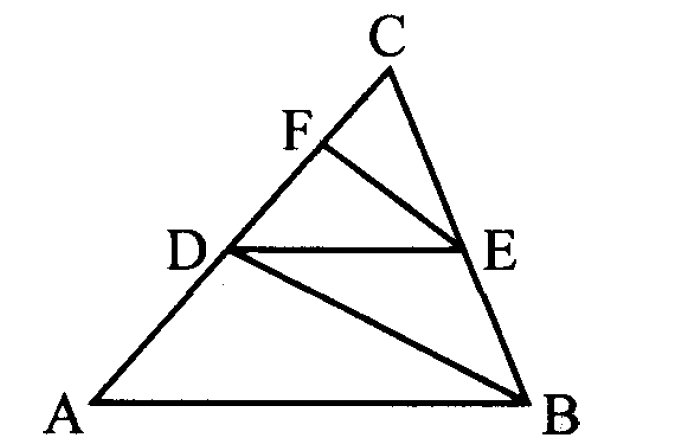
\includegraphics[width=5cm]{4.png}
 \end{figure}
 \item The mean of the following frequency distribution is 62.8. Find the missing frequency x.
 \begin{figure}[h!]
    \centering
    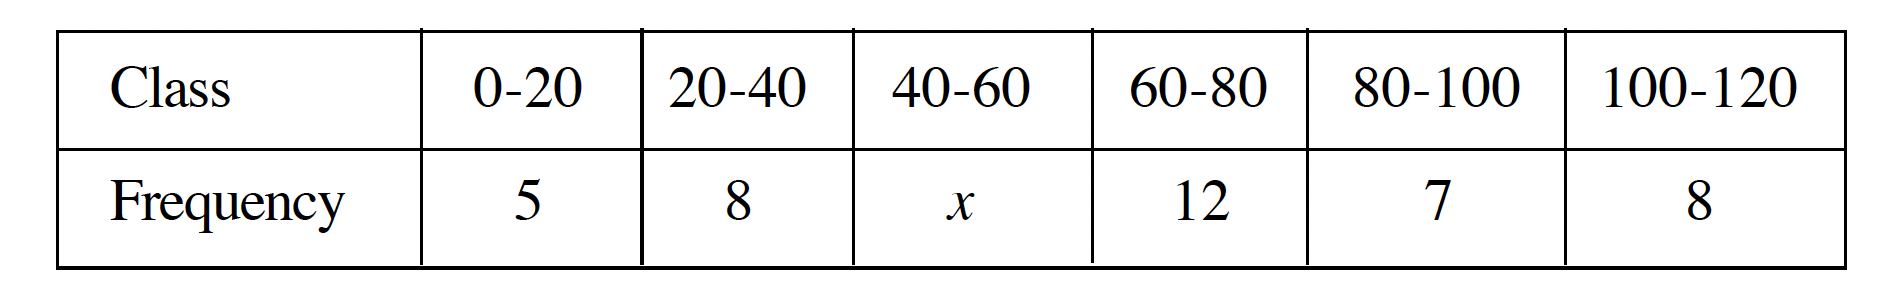
\includegraphics[width=10cm]{5.png}
 \end{figure}
 \medskip
\item Cards marked with numbers 3, 4, 5, ......, 50 are placed in a box and mixed thoroughly. One card is drawn at random from the box. Find the probability that number on the drawn card is
\begin{enumerate}
\item divisible by 7.
\item a number which is a perfect square.
\end{enumerate}
 \medskip
\item A washing machine is available for Rs. 13,500 cash or Rs. 6,500 as cash down payment followed by three monthly instalments of Rs. 2,500 each. Find the rate of interest charged under instalment plan.
\bigskip
\section{Section-B}
\item Solve the following system of equations graphically :
\begin{center}
2X+3Y=8 and X+4Y=9
\end{center}
\medskip
\item Simplify:
\begin{center}
$\displaystyle\frac{X}{X-Y}-\displaystyle\frac{Y}{X+Y}-\displaystyle\frac{2XY}{X^2-Y^2}$
\end{center}
\medskip
\item Which term of the A.P. 3, 15, 27, 39,....... will be 132 more than its $54^{th} $term ?
\medskip
\item In the blow figure, $\vec{TA}$ is a tangent to the circle from a point T and $\vec{TBC}$ is a secant to the circle. If $\vec{AD}$ is the bisector of $\measuredangle{CAB} $, prove that $\triangle{ADT} $ is isosceles.
\begin{figure}[h!]
    \centering
    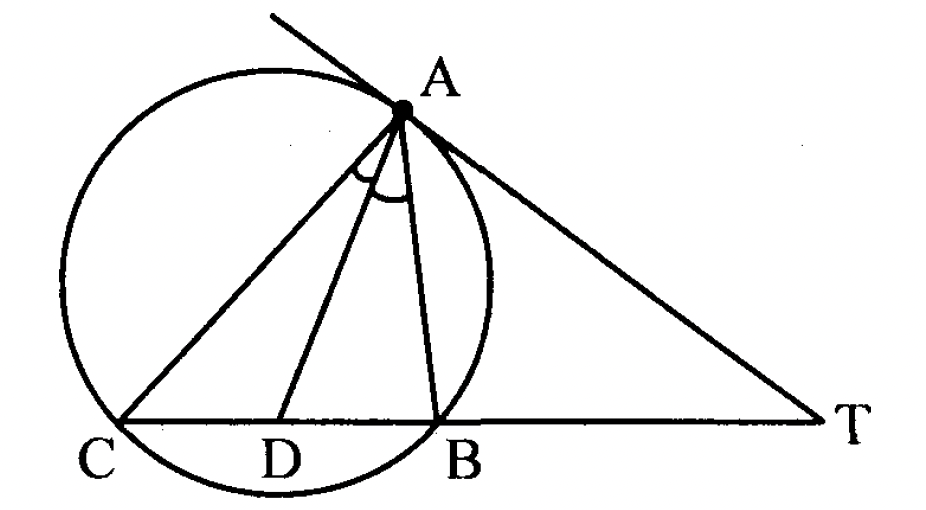
\includegraphics[width=5cm]{6.png}
 \end{figure}
 \medskip
 \item In  the $\triangle{ABC}$, $\vec{AD} \perp \vec{BC}$ and $\vec{AD^2}= \vec{BD}.\vec{DC}$.  Prove that $\measuredangle{BAC}$ is a right angle.
 \medskip 
 \item Draw a $\triangle{PQR}$ with the base $\vec{QR}$=6cm, vertical angle P= 60$\degree$ and median through $\vec{P}$ to the base is of length 4.5cm.
 \medskip
 \item A toy is in the form of a cone mounted on a hemisphere of common base radius 7 cm. The total height of the toy is 31 cm. Find the total surface area of the toy.
 \medskip
 \item The enrolment of a secondary school in different classes is given below. Draw a pie chart to represent the above data.
 \begin{figure}[h!]
    \centering
    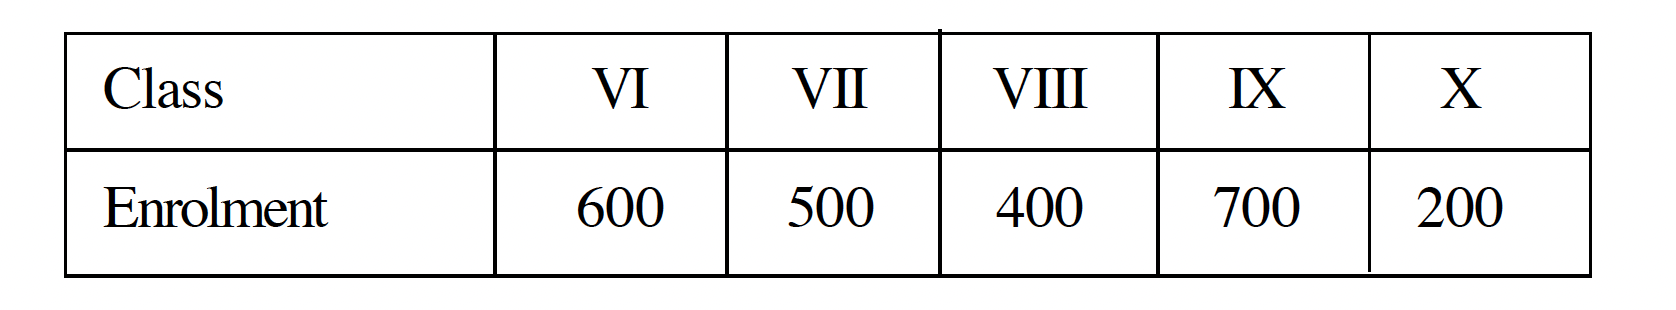
\includegraphics[width=10cm]{7.png}
 \end{figure}
 \medskip
 \item A bag contains 5 red balls and some blue balls. If the probability of drawing a blue ball from the bag is thrice that of a red ball, find the number of blue balls in the bag.
 \medskip
 \item Prove that
 \begin{center}
 $\displaystyle\frac{\cos A}{1-\tan A}+\displaystyle\frac{\sin A}{1-\cot A}=\sin A+\cos A$
 \end{center}
 \medskip
 \item Evaluate without using trigonometric tables :\\
 \bigskip
 $\displaystyle\frac{3\cos55\degree}{7\sin35\degree}+\displaystyle\frac{4(\cos70\degree.\cosec20\degree)}{7(\tan5\degree.\tan25\degree.\tan45\degree.\tan65\degree.\tan85\degree)}$
 \medskip
 \item Show that the points $\myvec{7,10} $, $\myvec{-2,5} $ and $\myvec{3,-4} $ are the vertices of an isosceles right triangle.
 \medskip
 \item In what ratio does the line X-Y-2=0 divides the line segment joining  $\myvec{3,-1} $ and  $\myvec{8,9} $? 
 \medskip
 \item A man borrows money from a finance company and has to pay it back in two equal half-yearly instalments of Rs. 7,396 each. If the interest is charged by the finance company at the rate of 15\%  per annum, compounded semi-annually, find the principal and the total interest paid.
 \bigskip
 \section{Section-C}
 \item If a line is drawn parallel to one side of a triangle, to intersect the other two sides in distinct points, prove that the other two sides are divided in the same ratio. Using the above, prove the following :\\ In the below figure, $\vec{DE} \| \vec{BC}$ and $\vec{BD}=\vec{CE}$. Prove that $\triangle{ABC}$ is an isosceles triangle.
 \begin{figure}[h!]
    \centering
    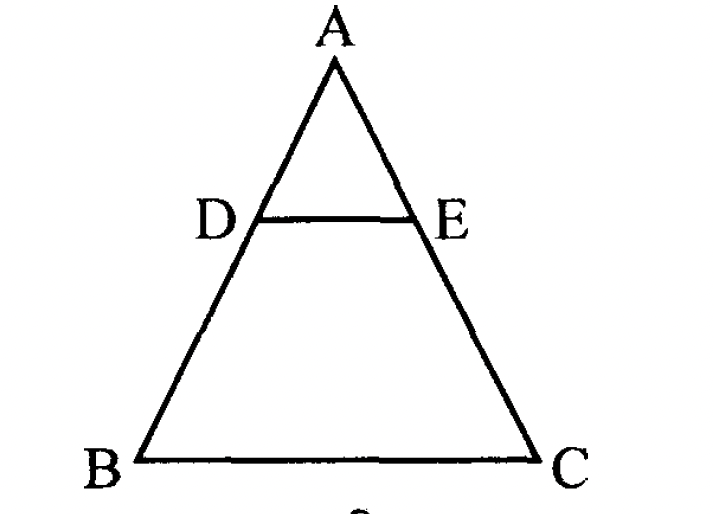
\includegraphics[width=5cm]{8.png}
 \end{figure}
 \medskip
 \item Prove that the sum of either pair of opposite angles of a cyclic quadrilateral is 180$\degree$. Using the above, find x and y in figure given below.
 \begin{figure}[h!]
    \centering
    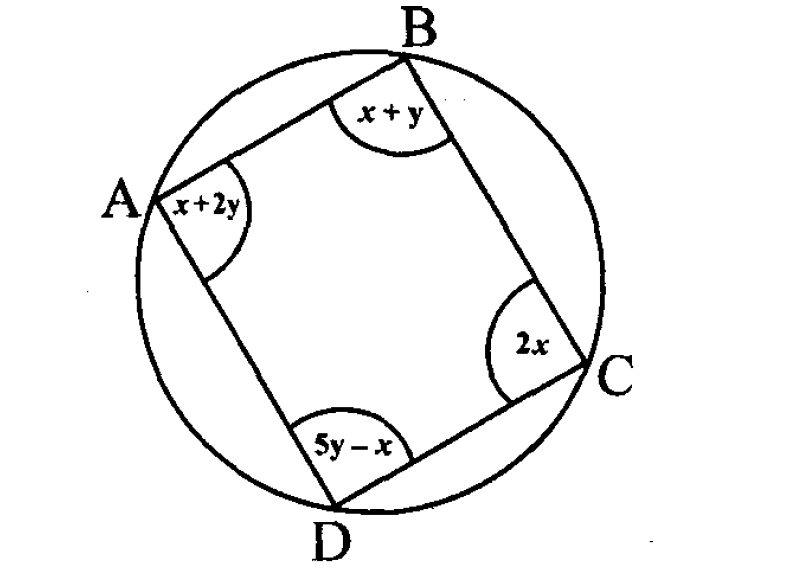
\includegraphics[width=5cm]{9.png}
 \end{figure}
 \medskip
 \item The difference of two numbers is 5 and the difference of their reciprocals is $\displaystyle\frac{1}{10}$. Find the numbers.
 \medskip
\item  By increasing the list price of a book by Rs. 10 a person can buy 10 less books for Rs. 1,200. Find the original list price of the book.
\medskip
\item A sphere, of diameter 12 cm, is dropped in a right circular cylindrical vessel, partly filled with water. If the sphere is completely submerged in water, the water level in the cylindrical vessel rises by {3}$\dfrac{5}{9}$ cm. Find the diameter of the cylindrical vessel.
\medskip
\item A solid right circular cone of diameter 14 cm and height 8 cm is melted to form a hollow sphere. If the external diameter of the sphere is 10 cm, find the internal diameter of the sphere.
\medskip
\item A boy standing on a horizontal plane finds a bird flying at a distance of 100 m from him at an elevation of 30$\degree$. A girl standing on the roof of 20 metre high building, finds the angle of elevation of the same bird to be 45$\degree$. Both the boy and the girl are on opposite sides of the bird. Find the distance of bird from the girl.
\medskip
\item Ms. Shahnaz earns Rs. 35,000 per month (excluding HRA). She donates Rs. 30,000 to Prime Minister Relief Fund (100\% exemption) and Rs. 40,000 to a Charitable Hospital (50\% exemption). She contributes Rs. 5,000 per month to Provident Fund and Rs. 25,000 per annum towards LIC premium. She purchases NSC worth Rs. 20,000. She pays Rs. 2,300 per month towards income tax for 11 month. Find the amount of income tax she has to pay in 12th month of the year.\\
Use the following to calculate income tax :\\
\begin{figure}[h!]
    \centering
    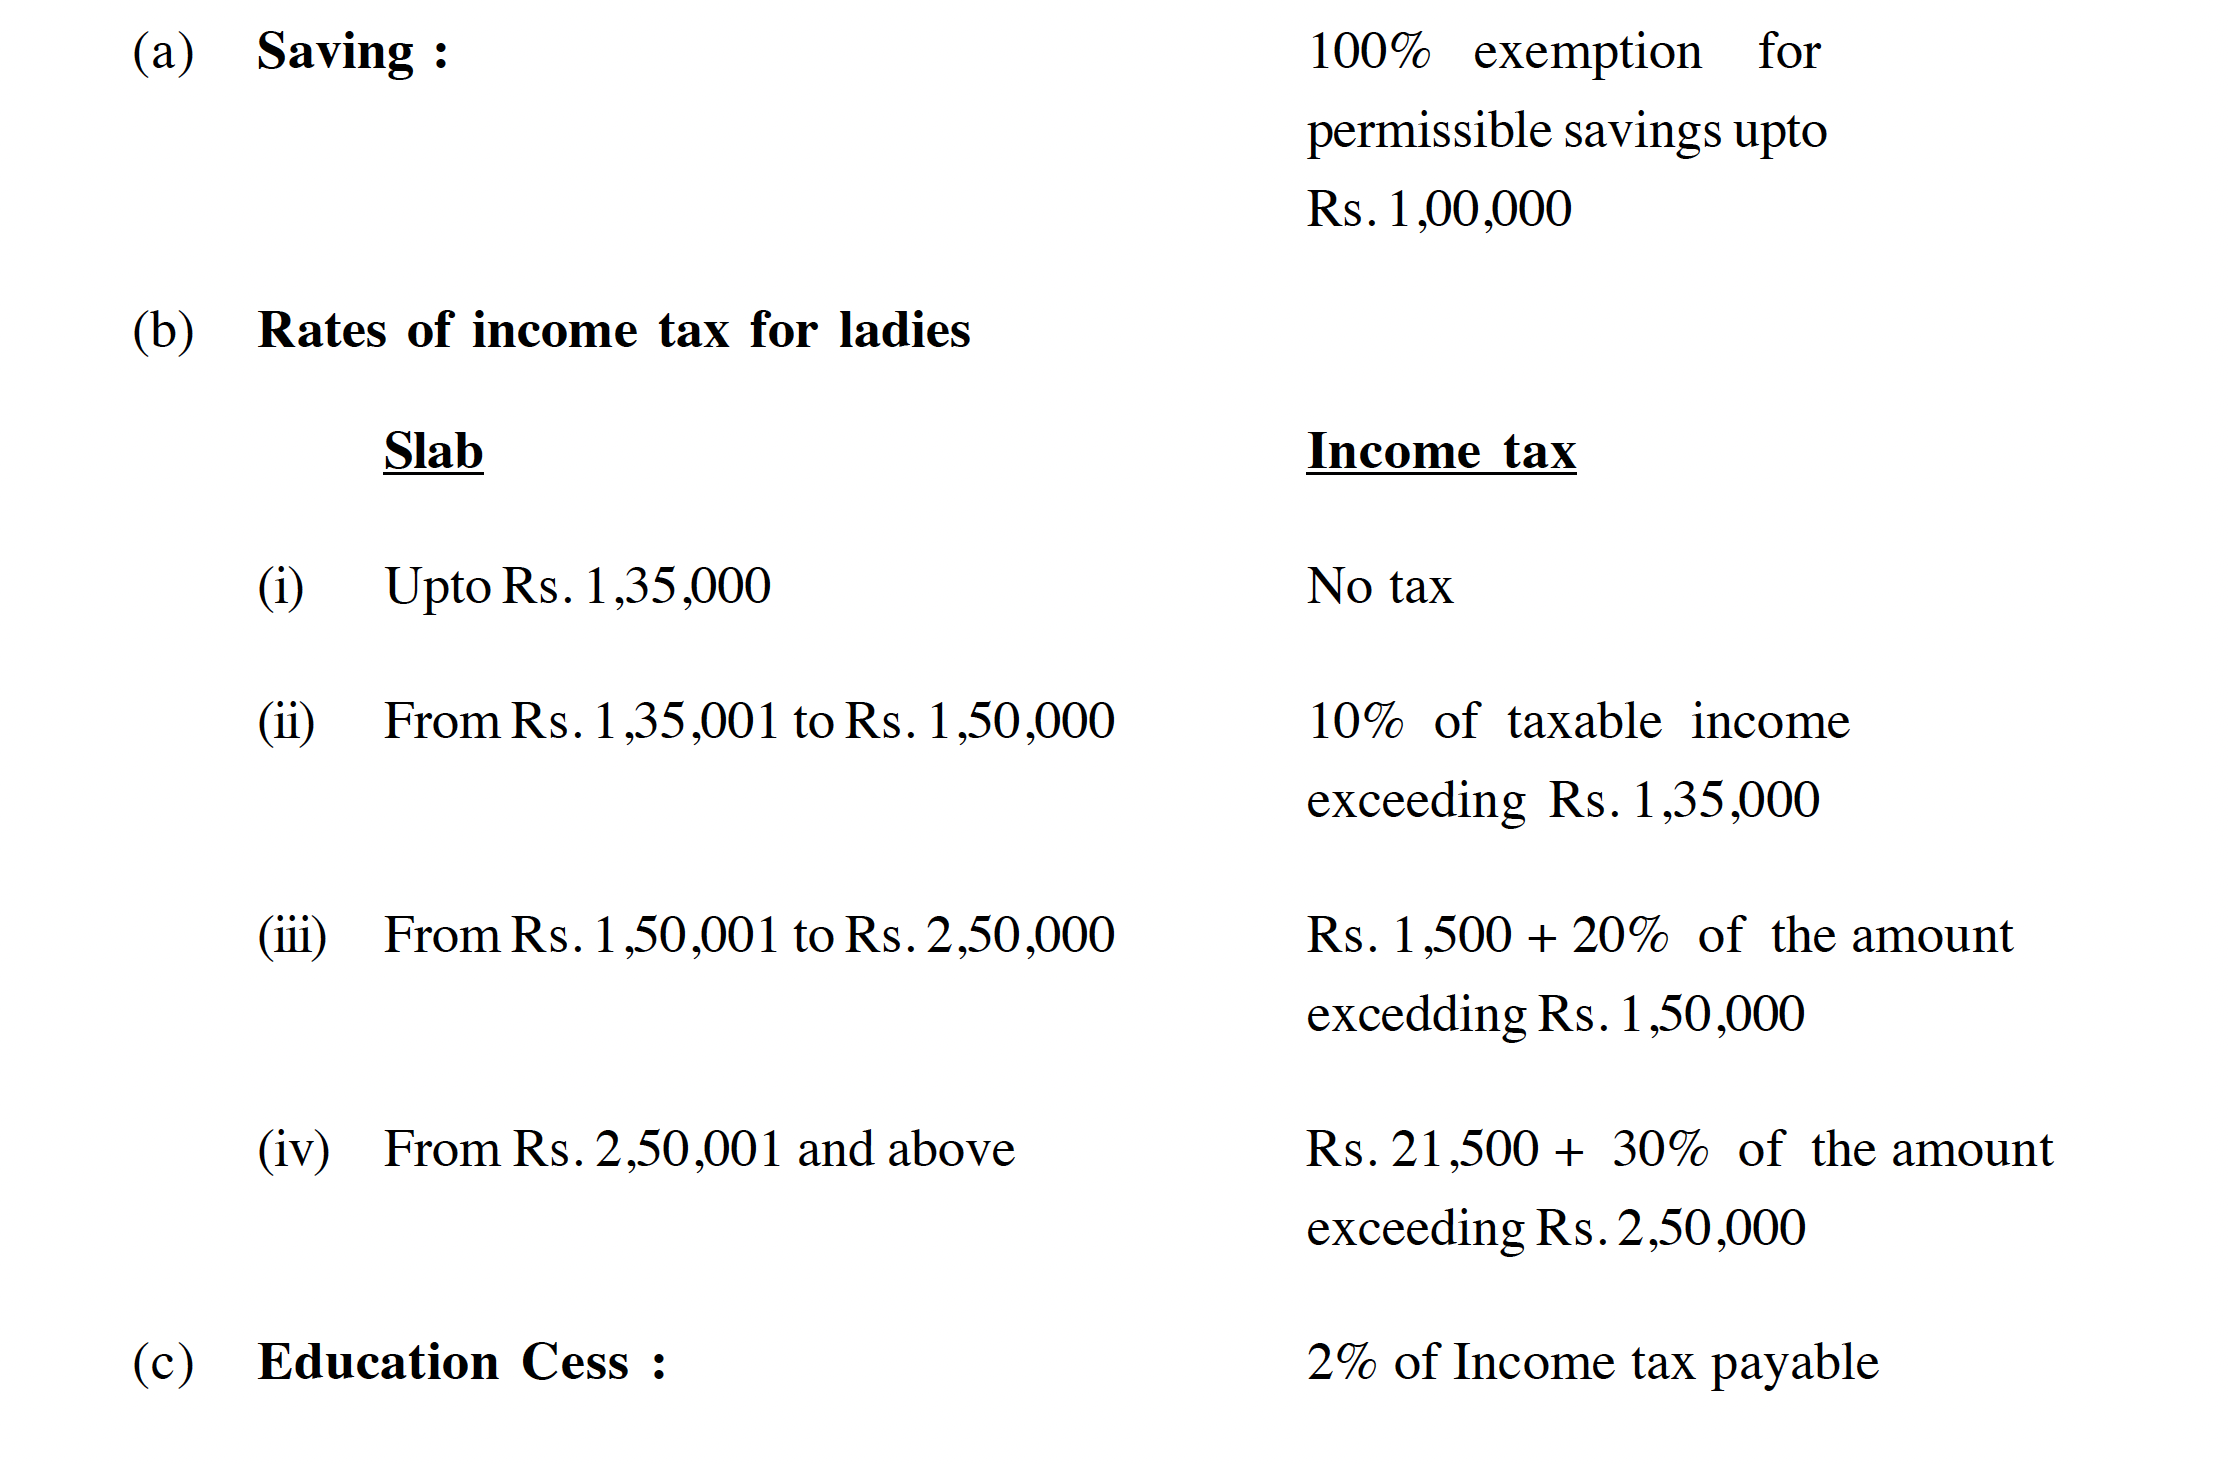
\includegraphics[width=10cm]{10.png}
 \end{figure}
 \end{enumerate}


\end{document}